\section{Ocean dynamics}
% =========================================
% =========================================




\begin{frame}{Ocean dynamics}
	\framesubtitle{Hydrostatics}
	\begin{tikzpicture}[remember picture,overlay]
		% \node[fill=blue!30, text=white, font=\large, rounded corners] 
		\node at (current page.north east) [xshift=-3.8cm, yshift=-3cm] 
		{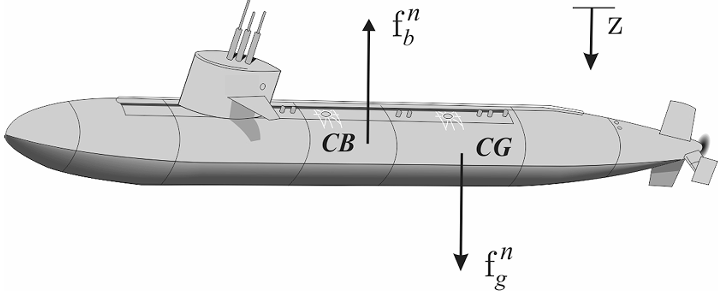
\includegraphics[width=0.7\linewidth]{img/force.png}};
	\end{tikzpicture}
	
	\vspace{1cm}
	
	Forces act in the vertical plane 
	\begin{align}
		f_g^n = \begin{bmatrix}
			0 & 0 & W
		\end{bmatrix}^\top; \quad f_b^n = -\begin{bmatrix}
			0 & 0 & B
		\end{bmatrix}^\top
	\end{align}
	Thus, the gravity vector is
	\begin{align}
		{g}(\eta) &= - 
		\begin{bmatrix}
			{f}_g^b + {f}_b^b \\
			{r}_g^b \times {f}_g^b + {r}_b^b \times {f}_b^b
		\end{bmatrix} \\
		&= - 
		\begin{bmatrix}
			{R}_b^n (\Theta_{nb})^{-1} \left( {f}_g^n + {f}_b^n \right) \\
			{r}_g^b \times {R}_b^n (\Theta_{nb})^{-1} {f}_g^n + 
			{r}_b^b \times {R}_b^n (\Theta_{nb})^{-1} {f}_b^n
		\end{bmatrix}.
	\end{align}
	\textbf{Note:} These formulations become more complex when considering the surface vessels
\end{frame}



% =========================================
% =========================================



\begin{frame}{Ocean dynamics}
	\framesubtitle{Seakeeping Theory(wave and wind)}
	\begin{block}{Vehicle-Ocean dynamics model}
		\begin{align}
			\dot{\eta} = J_{\Theta}(\eta)\nu \notag \\
			M_{RB} \dot{\nu} + C_{RB}^* \nu + M_A \dot{\nu}_r + C_A^* \nu_r + (D_P + D_V) \nu_r + \mu + G \eta + g_o = \tau_{\text{wind}} + \tau_{\text{wave}}  + \tau  \notag
		\end{align}
	\end{block}
	\begin{block}{Vehicle-Ocean dynamics model}
		\begin{align}
			\text{Inertia forces:} & \quad M_{RB} \dot{\nu} + C_{RB}^* \nu + M_A \dot{\nu}_r + C_A^* \nu_r \notag\\
			\text{Damping forces:} & \hspace{1.8cm} + (D_P + D_V) \nu_r + \mu \notag\\
			\text{Restoring forces:} & \hspace{3.3cm} + G \eta + g_o \notag\\
			\text{Wind and wave forces:} & \hspace{5cm} = \tau_{\text{wind}} + \tau_{\text{wave}} \notag\\
			\text{Propulsion forces:} & \hspace{5.5cm} + \tau \notag
		\end{align}
	\end{block}
\end{frame}

% =========================================
% =========================================


\begin{frame}{Ocean dynamics}
	\framesubtitle{Seakeeping kinematics (wave and wind)}
	\begin{tikzpicture}[remember picture,overlay]
		% \node[fill=blue!30, text=white, font=\large, rounded corners] 
		\node at (current page.north east) [xshift=-4cm, yshift=-4cm] 
		{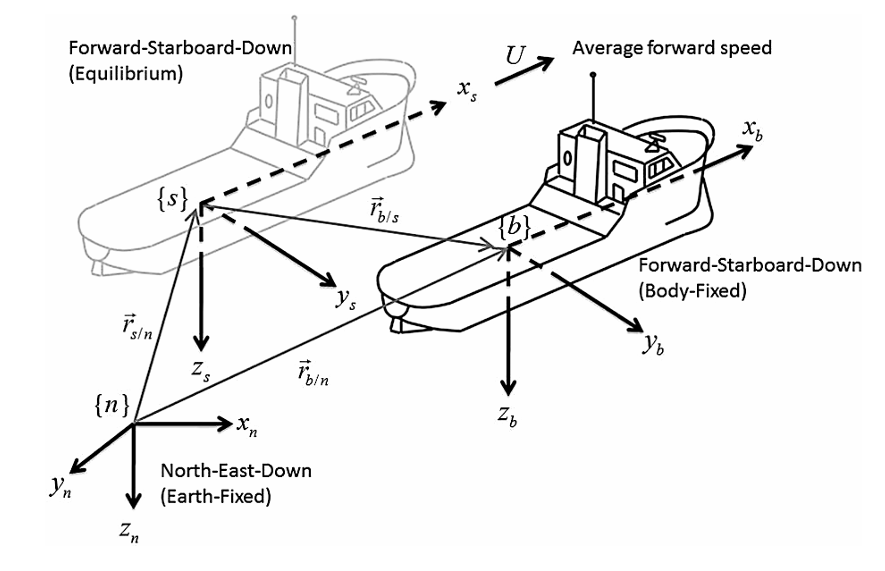
\includegraphics[width=0.7\linewidth]{img/seakeeping.png}};
	\end{tikzpicture}
	
	\vspace{4cm}
	
	Several notations
	\begin{itemize}
		\item $v_{s/n}^n = \begin{bmatrix}
			U\cos{\bar{\psi}} & U\sin{\bar{\psi}} & 0
		\end{bmatrix}^\top$
		\item $\omega_{s/n}^n = \begin{bmatrix}
			0 & 0 & 0
		\end{bmatrix}^\top$
		\item $\Theta_{ns} = \begin{bmatrix}
			0 & 0 & \bar{\psi}
		\end{bmatrix}^\top$
	\end{itemize}
	
\end{frame}


% =========================================
% =========================================


\begin{frame}{Ocean dynamics}
	\framesubtitle{Seakeeping kinematics(wave and wind)}
	Define the perturbation coordinate
	\begin{align}
		\delta\eta = \begin{bmatrix}
			r_{b/s}^s \\ \Theta_{sb}
		\end{bmatrix}; \quad \delta \nu = \begin{bmatrix}
			v_{b/s}^b \\ \omega_{b/s}^b
		\end{bmatrix} ; \quad \xi = \delta \eta; \quad \Theta_{sb} = \begin{bmatrix}
			\delta\phi \\ \delta\theta \\ \delta\psi
		\end{bmatrix}
	\end{align}
	Thus, the following equations are achieved as the transformation between BODY and SEAKEEPING coordinates
	\begin{block}{Transformation between BODY and SEAKEEPING}
		\begin{align}
			\dot{\nu} = -UL\delta\nu + \delta\dot{\nu}
		\end{align}
		where $U$ is the velocity of the vehicle and $L \in \mathbb{R}_{6\times 6}$\\
		\textbf{Linear transformations}
		\begin{align}
			\delta\nu \approx \nu + U(L\delta\eta - e_1)\\
			\delta\dot{\nu} \approx \dot{\nu} + UL\nu
		\end{align}
	\end{block}
\end{frame}



% =========================================
% =========================================



\begin{frame}{Ocean dynamics}
	\framesubtitle{Added mass(wave and wind)}
	From Cummins Equation in SEAKEEPING Coordinates, the following equations are introduced
	\begin{block}{Frequency-domain seakeeping equation of motion}
		\begin{align}
			\Big(-\omega^2(M_{RB} + \bar{A}(\omega
			)) - j\omega B(\omega) + C
			\Big)\ddot{\xi}(j\omega
			)= \tau_{wind}(j\omega)+ \tau_{wave}(j\omega) + \delta\tau(j\omega)
		\end{align}
	\end{block}
	
	\begin{block}{Time-domain seakeeping equation of motion}
		\begin{align}
			\Big(M_{RB} + \bar{A}\Big)\ddot{\xi} + \int\limits_{-\infty}^t \bar{K}(t - \tau)\dot{\xi}(t)d\tau + \bar{C}\xi = \tau_{wind} + \tau_{wave} + \delta\tau
		\end{align}
	\end{block}
	where $\bar{K} = \dfrac{2}{\pi}\int\limits_{0}^{\infty}B(\omega)\cos(\omega t)d\omega$
	
	\textbf{Notice:} For underwater vehicle, $A(\omega) = \text{const}$ and $B(\omega) = 0$
\end{frame}



% =========================================
% =========================================


\begin{frame}{Ocean dynamics}
	\framesubtitle{Added mass(wave and wind)}
	\begin{block}{Hydrodynamic added mass forces and moments in 6 DOFs}
		\begin{itemize}
			\item The expressions are complicated and not suited for control design.
			\item Hydrodynamic software programs such as WAMIT and ShipX can be used to compute the added mass term.
		\end{itemize}
	\end{block}
	\vspace{4cm}
	
	\begin{tikzpicture}[remember picture,overlay]
		% \node[fill=blue!30, text=white, font=\large, rounded corners] 
		\node at (current page.north west) [xshift=3cm, yshift=-6.5cm] {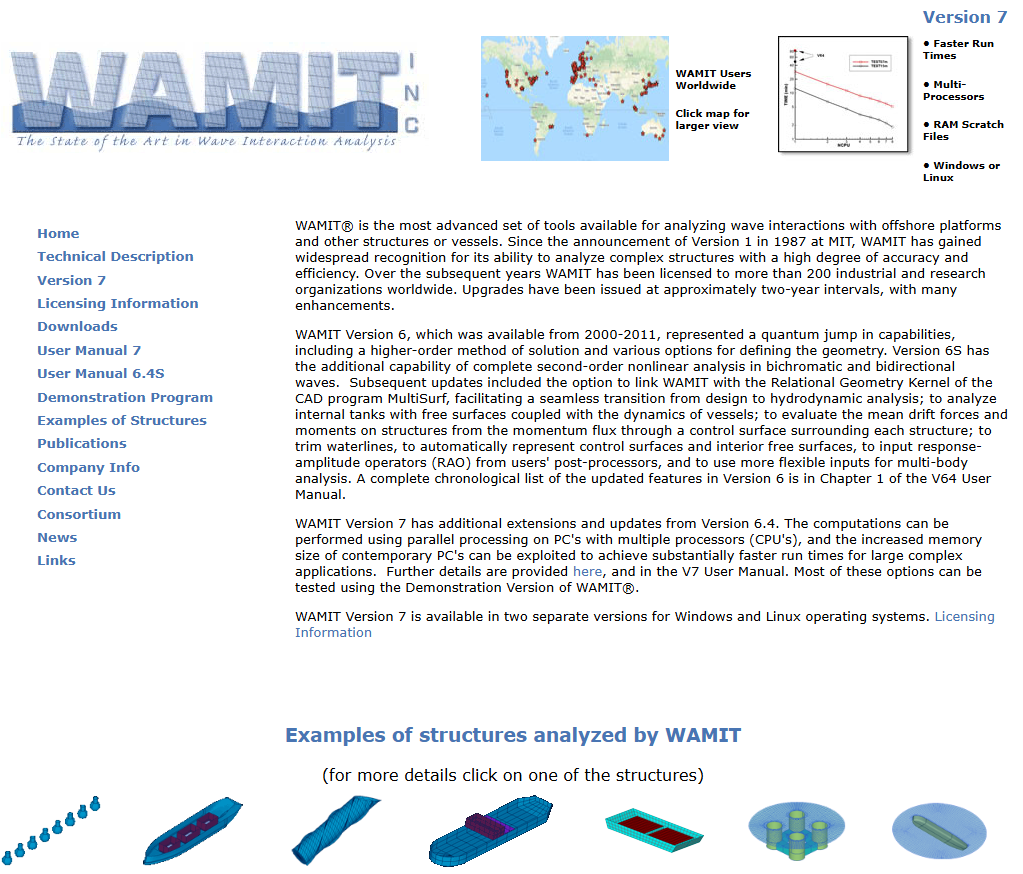
\includegraphics[width=0.4\linewidth]{img/wamit.png}};
	\end{tikzpicture}
	
	\begin{tikzpicture}[remember picture,overlay]
		% \node[fill=blue!30, text=white, font=\large, rounded corners] 
		\node at (current page.north west) [xshift=9.5cm, yshift=-6.5cm] {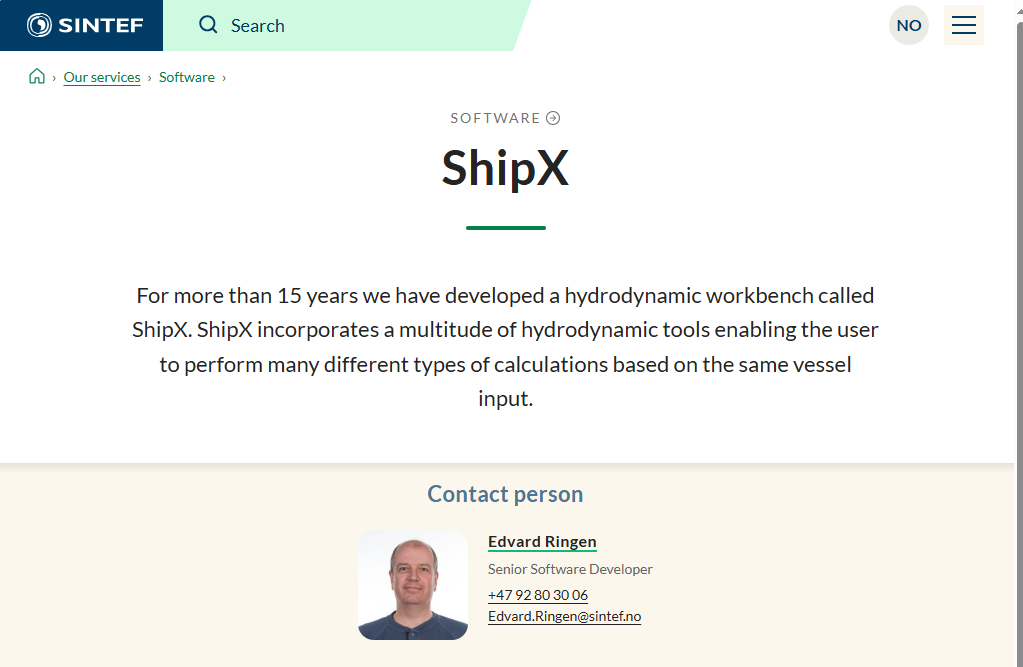
\includegraphics[width=0.5\linewidth]{img/shipX.png}};
	\end{tikzpicture}
\end{frame}


% =========================================
% =========================================


\begin{frame}{Ocean dynamics}
	\framesubtitle{Linear equation of motion}
	From Cummins Equation in SEAKEEPING Coordinates, the following equations are introduced
	\begin{block}{Linear equation of motion (Zero-Speed Potential Coefficients)}
		\begin{align}
			M\dot{\nu} + C_{RB}^*\nu + C_A^*\nu_r + D\nu_r + \int\limits_0^tK(t-\tau)[\nu(\tau) - Ue_1]d\tau + G\eta = \sum\tau
		\end{align}
	\end{block}
	\begin{block}{Linear equation of motion (Speed-Dependent Potential Coefficients)}
		\begin{align}
			M_U\dot{\nu} + C_{RB}^*\nu + C_A^*\nu_r + D_U\nu_r + \int\limits_0^tK_U(t-\tau)[\nu(\tau) - Ue_1]d\tau + G\eta = \sum\tau
		\end{align}
	\end{block}
	where $\sum\tau = \tau_{wind} + \tau_{wind} + \tau$
\end{frame}


% =========================================
% =========================================


\begin{frame}{Ocean dynamics}
	\framesubtitle{Maneuvering Theory}
	\begin{block}{Goal}
		\begin{align}
			\underbrace{{M_{RB} \dot{\nu} + C_{RB}(\nu) \nu}}_{\text{rigid-body forces}} + 
			\underbrace{{M_A \dot{\nu}_r + C_A(\nu_r) \nu_r + D(\nu_r) \nu_r}}_{\text{hydrodynamic forces}}
			+\underbrace{{g(\eta) + g_o}}_{\text{hydrostatic forces}}
			= \tau + \tau_{\text{wind}} + \tau_{\text{wave}}
		\end{align}
		or
		\begin{align}
			M \dot{\nu}_r + C(\nu_r) \nu_r + D(\nu_r) \nu_r + g(\eta) + g_o = \tau + \tau_{\text{wind}} + \tau_{\text{wave}}
		\end{align}
		where $\nu_r = \nu - \nu_c$ is the relative velocity vector.
	\end{block}
	\begin{itemize}
		\item For slender bodies, such as AUV, the longitudinal (surge, heave, and pitch motion) and lateral (sway, roll, and yaw motion) models are referred to consider.
		\item For ROVs operating, the horizontal-plane (surge, sway, and yaw motion) and depth (heavy) models are referred to consider.
	\end{itemize}
\end{frame}




% =========================================
% =========================================


\begin{frame}{Ocean dynamics}
	\framesubtitle{Maneuvering Theory - 3DOF maneuvering model}
	\begin{block}{3DOF maneuvering model}
		The horizontal motions (surge, sway, and heave) of a marine craft moving at forward speed could be described by a zero frequency model, where
		\begin{align}
			M_A = \begin{bmatrix}
				A_{11}(0) & 0 & 0 \\
				0 & A_{22}(0) & A_{26}(0) \\
				0 & A_{62}(0) & A_{66}(0)
			\end{bmatrix}\\
			D_p = 0
		\end{align}
		are the constant matrices.
	\end{block}
	\textbf{Limitation}  One limitation of the zero-frequency assumption is that it cannot be applied to heave, roll, and pitch.  For 2nd-order mass-damper-spring systems the dominating frequencies are the natural frequencies.
\end{frame}


% =========================================
% =========================================


\begin{frame}{Ocean dynamics}
	\framesubtitle{Extension to 6-DOF models}
	\begin{block}{Extension to 6-DOF models}
		\textbf{Solution:} Formulate frequency-independent models in heave, pitch, and roll at their respective natural frequencies and not the zero frequency.
		\begin{align}
			\omega_3 = \sqrt{\dfrac{C_{33}}{m + A_{33}(\omega_3)}}\\
			\omega_4 = \sqrt{\dfrac{C_{44}}{I_x + A_{44}(\omega_4)}}\\
			\omega_5 = \sqrt{\dfrac{C_{55}}{I_y + A_{55}(\omega_5)}}
		\end{align}
	\end{block}
	\textbf{Key assumption:} No coupling between the surge-sway-yaw and the heave-roll-pitch subsystems.
\end{frame}



% =========================================
% =========================================


\begin{frame}{Ocean dynamics}
	\framesubtitle{Added Mass Forces in a Rotating Coordinate System}
	The expression for the fluid kinetic energy \( T_A \), see Ref. \footnote{Imlay, Frederick H. \textit{The complete expressions for added mass of a rigid body moving in an ideal fluid}. No. Report 1528. 1961.}, can be written as a quadratic form of the body axis velocity vector components, that is:
	\begin{align}
		T_A = \frac{1}{2} \boldsymbol{\nu}^T M_A \boldsymbol{\nu}
	\end{align}
	
	Here \( M_A \) is a \( 6 \times 6 \) added inertia matrix defined as:
	\begin{align}
		M_A = 
		\begin{bmatrix}
			A_{11} & A_{12} \\
			A_{21} & A_{22}
		\end{bmatrix}
		\triangleq - 
		\begin{bmatrix}
			X_{\dot{u}} & X_{\dot{v}} & X_{\dot{w}} & X_{\dot{p}} & X_{\dot{q}} & X_{\dot{r}} \\
			Y_{\dot{u}} & Y_{\dot{v}} & Y_{\dot{w}} & Y_{\dot{p}} & Y_{\dot{q}} & Y_{\dot{r}} \\
			Z_{\dot{u}} & Z_{\dot{v}} & Z_{\dot{w}} & Z_{\dot{p}} & Z_{\dot{q}} & Z_{\dot{r}} \\
			K_{\dot{u}} & K_{\dot{v}} & K_{\dot{w}} & K_{\dot{p}} & K_{\dot{q}} & K_{\dot{r}} \\
			M_{\dot{u}} & M_{\dot{v}} & M_{\dot{w}} & M_{\dot{p}} & M_{\dot{q}} & M_{\dot{r}} \\
			N_{\dot{u}} & N_{\dot{v}} & N_{\dot{w}} & N_{\dot{p}} & N_{\dot{q}} & N_{\dot{r}}
		\end{bmatrix}, \quad Y_A = Y_{\dot{u}}\dot{u}, \quad Y_{\dot{u}} \triangleq \dfrac{\partial Y}{\partial \dot{u}}
	\end{align}
	\textbf{Notice:} In a real fluid, these 36 constants could be distinct. With ideal (without friction),$M_A = M_A^\top$
\end{frame}



% =========================================
% =========================================


\begin{frame}{Ocean dynamics}
	\framesubtitle{Added Mass Forces in a Rotating Coordinate System}
	\begin{block}{Hydrodynamic Coriolis-Centripetal Matrix $C_A(\nu)$}
		For a rigid body moving through an ideal fluid the hydrodynamic Coriolis and centripetal matrix $C_A(\nu)$ could always be parametrized such that it is skew-symmetric
		\begin{align}
			C_A(\nu) = -C_A(\nu)^\top, \quad \forall\nu
		\end{align}
		As mentioned above,
		\begin{align}
			C_A(\nu) = \begin{bmatrix}
				0 & -S(A_{11}\nu_1 + A_{12}\nu_2) \\
				-S(A_{11}\nu_1 + A_{12}\nu_2) & -S(A_{21}\nu_1 + A_{22}\nu_2) 
			\end{bmatrix}
		\end{align}
	\end{block}
\end{frame}

% =========================================
% =========================================



\begin{frame}{Ocean dynamics}
	\framesubtitle{Added Mass Forces in a Rotating Coordinate System}
	\begin{block}{Vehicle-Ocean dynamics model}
		\begin{align}
			\dot{\eta} = J_{\Theta}(\eta)\nu \notag \\
			M_{RB} \dot{\nu} + C_{RB}^* \nu + M_A \dot{\nu}_r + C_A^* \nu_r + (D_P + D_V) \nu_r + \mu + G \eta + g_o = \tau_{\text{wind}} + \tau_{\text{wave}}  + \tau  \notag
		\end{align}
	\end{block}
	\begin{block}{Vehicle-Ocean dynamics model}
		\begin{align}
			\text{Inertia forces:} & \quad M_{RB} \dot{\nu} + C_{RB}^* \nu + M_A \dot{\nu}_r + C_A^* \nu_r \notag\\
			\text{Damping forces:} & \hspace{1.8cm} + (D_P + D_V) \nu_r + \mu \notag\\
			\text{Restoring forces:} & \hspace{3.3cm} + G \eta + g_o \notag\\
			\text{Wind and wave forces:} & \hspace{5cm} = \tau_{\text{wind}} + \tau_{\text{wave}} \notag\\
			\text{Propulsion forces:} & \hspace{5.5cm} + \tau \notag
		\end{align}
	\end{block}
\end{frame}




% =========================================
% =========================================




\begin{frame}{Ocean dynamics}
	\framesubtitle{Viscous damping}
	In practical implementations, it is difficult to determine higher-order terms as well as the off-diagonal terms in general expression for hydrodynamic damping.
	
	The different damping terms contribute to both linear and quadratic damping. However, it is in general difficult to separate these effects. In many cases, it is convenient to write total hydrodynamic damping as
	\begin{align}
		D(\nu_r) = D + D_n(\nu_r)
	\end{align}
	\begin{itemize}
		\item Linear viscous damping
		\begin{align}
			D = D_p + D_v \approx -diag(X_u, Y_v, Z_w, K_p, M_q, N_r)
		\end{align}
		\item Nonlinear surge damping
		\begin{itemize}
			\item Nonlinear Surge Damping: Damping Due to Vortex Shedding
			\item Cross-Flow Drag Principle (lifting Forces:): For relative current angles, the cross-flow drag principle may be applied to calculate the nonlinear damping force in sway and the yaw moment
		\end{itemize}
	\end{itemize}
\end{frame}






% =========================================
% =========================================




\begin{frame}{Ocean dynamics}
	\framesubtitle{Linear viscous damping}
	The approximate diagonal matrix $D_p$ is expressed as:
	
	\begin{equation}
		D_p \approx 
		\begin{bmatrix}
			0 & 0 & 0 & 0 & 0 & 0 \\
			0 & 0 & 0 & 0 & 0 & 0 \\
			0 & 0 & B_{33}(\omega_\text{heave}) & 0 & 0 & 0 \\
			0 & 0 & 0 & B_{44}(\omega_\text{roll}) & 0 & 0 \\
			0 & 0 & 0 & 0 & B_{55}(\omega_\text{pitch}) & 0 \\
			0 & 0 & 0 & 0 & 0 & 0
		\end{bmatrix} 
	\end{equation}
	
	The natural frequencies $\omega_\text{heave}$, $\omega_\text{roll}$, and $\omega_\text{pitch}$ can be computed as introduced in the above.
	
	A diagonal matrix usually approximates the linear viscous damping terms:
	\begin{equation}
		D_v \approx \text{diag}\{B_{11v}, B_{22v}, B_{33v}, B_{44v}, B_{55v}, B_{66v}\}
	\end{equation}
	
	where the elements $B_{iiv} \; (i = 1, \ldots, 6)$ can be computed from the time constants and natural periods of the system (see Section 6.4).
\end{frame}




% =========================================
% =========================================



\begin{frame}{Ocean dynamics}
	\framesubtitle{Linear viscous damping}
	The expressions for the diagonal elements of $D_v$ are as follows:
	\begin{align}
		B_{11v} &= \frac{m + A_{11}(0)}{T_\text{surge}} = \frac{8\pi \zeta_\text{surge}[m + A_{11}(0)]}{T_{n,\text{surge}}} \\
		B_{22v} &= \frac{m + A_{22}(0)}{T_\text{sway}} = \frac{8\pi \zeta_\text{sway}[m + A_{22}(0)]}{T_{n,\text{sway}}} \\
		B_{33v} &= 2\Delta \zeta_\text{heave} \omega_\text{heave} [m + A_{33}(\omega_\text{heave})] \\
		B_{44v} &= 2\Delta \zeta_\text{roll} \omega_\text{roll} [I_x + A_{44}(\omega_\text{roll})] \\
		B_{55v} &= 2\Delta \zeta_\text{pitch} \omega_\text{pitch} [I_y + A_{55}(\omega_\text{pitch})] \\
		B_{66v} &= \frac{I_z + A_{66}(0)}{T_\text{yaw}} = \frac{8\pi \zeta_\text{yaw}[I_z + A_{66}(0)]}{T_{n,\text{yaw}}}
	\end{align}
\end{frame}




% =========================================
% =========================================





\begin{frame}{Ocean dynamics}
	\framesubtitle{Nonlinear viscous damping}
	\begin{block}{Quadratic drag and lifting in 6DOF}
		Quadratic drag and lifting in 6DOF
		\begin{align}
			D_n(\nu_r)\nu_r = [|\nu_r|^\top D_i(\rho, A, C_D)\nu_r)]_{6\times1}
		\end{align}
		The viscous damping force due to vortex shedding can be modeled as
		\begin{align}
			f(U) = -\dfrac{1}{2}\rho C_D A |U_r|U_r
		\end{align}
		where $\rho$ is the fluid density, $C_D$ is drag coefficient, $A$ is the projected cross-sectional area, and $U$ is the velocity of the vehicle.
	\end{block}
\end{frame}




% =========================================
% =========================================



\begin{frame}{Ocean dynamics}
	\framesubtitle{Maneuvering Equations}
	
	\textbf{{Hydrodynamic Mass--Damper}}
	
	\begin{itemize}
		\item \textbf{Added mass} $M_A$ due to the inertia of the surrounding fluid (see Section 6.2). The corresponding Coriolis and centripetal matrix due to added mass is due to the rotation of $\{b\}$ with respect to $\{n\}$ and is denoted $C_A({v}_r)$ (see Section 6.3).
		\item \textbf{Radiation-induced potential damping} $D_p$ due to the energy carried away by generated surface waves.
		\item \textbf{Viscous damping} caused by skin friction, wave drift damping, vortex shedding, and lift/drag (see Section 6.4). 
	\end{itemize}
	The resulting hydrodynamic force is written as:
	\begin{align}
		{\tau}_\text{hyd} = -M_A \dot{\nu}_r - C_A(\nu_r) \nu_r - D_p \nu_r + {\tau}_\text{visc}
	\end{align}
	where $\nu_r = \nu - \nu_c$ with $\nu_c = [u_c, v_c, w_c, 0, 0, 0]^\top$ is the relative velocity due to an \textit{irrotational constant ocean current} (see Section 8.3), and
	\begin{align}
		{\tau}_\text{visc} = -D_v {v}_r - D_n({v}_r) {v}_r
	\end{align}
	\textbf{{Hydrostatic Spring Stiffness}}: \textbf{Restoring forces} due to Archimedes
	\begin{align}
		{\tau}_\text{hs} = -g({\eta}) - {g}_o
	\end{align}
\end{frame}


% =========================================
% =========================================


